
\section{Introduction}

MacSim is a heterogeneous architecture simulator, specifically supporting x86 ISA and NVIDIA PTX ISA. It is a trace-driven cycle-level simulator.  It can simulate homogeneous ISA multicore simulations, heterogeneous ISA multicore simulations. It uses Ocelot for PTX trace generation and Pin to generate x86 traces. Both traces are converted internal RISC style uops and those uops are simulated. MacSim is a microarchitecture simulator that simulates detailed pipeline (in-order and out-of-order) and a memory system including caches, NoC, memory controllers. It supports, asymmetric multicore configurations (small cores + medium cores+ big cores ) and SMT or MT architectures as well. 

Currently interconnection network model (based on IRIS) and power model (based on McPat) are connected. ARM ISA support is on-progress. MacSim is also one of the components of SST so multiple MacSim simulators can run concurrently. 

\begin{figure*}[htb]
\centering
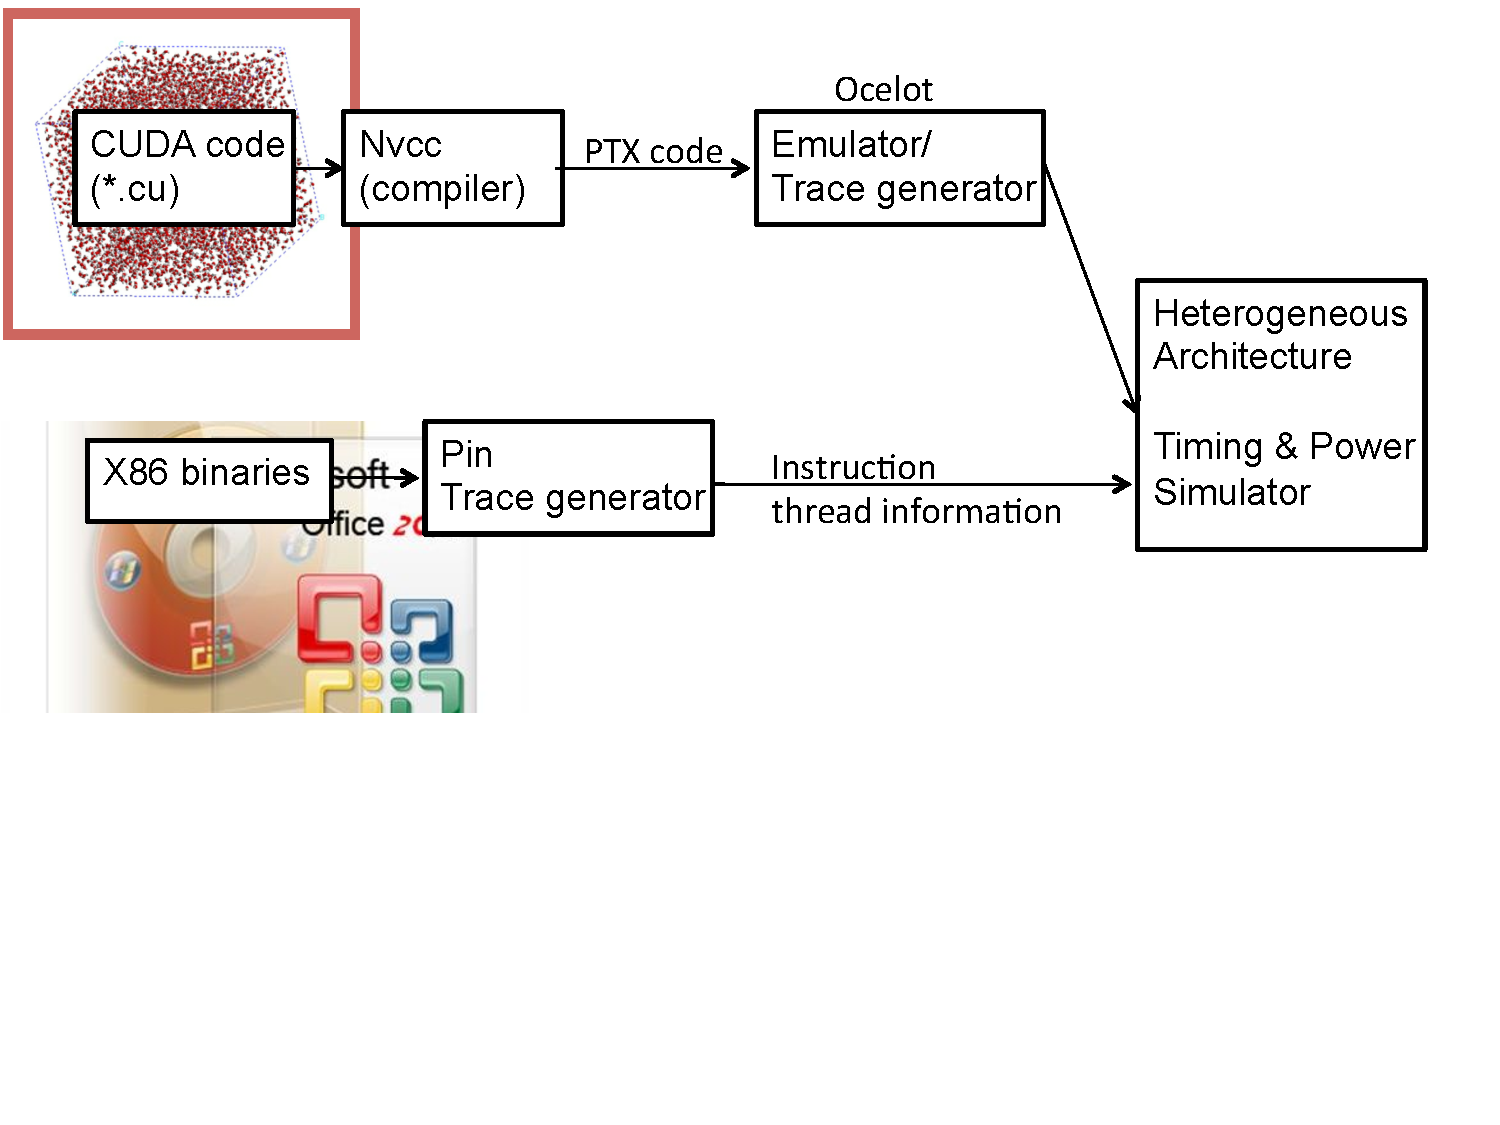
\includegraphics[width=5in]{fig/macsim_overview}
\caption{The overview of MacSim Simulator}
\label{fig:overview}
\end{figure*}



% LocalWords:  Macsim MacSim NVIDIA PTX multicore RISC uops microarchitecture
% LocalWords:  NoC SMT McPat
